\chapter{Design and Implementation}\label{C:workdone}

\section{Overview}

\todo{REDO ONCE FINISHED SECTION}
The ability to trace java unit tests and perform several different analysis metrics has been implemented. For this to be achieved, several factors had to be completed and these are explored in this chapter. The different types of spectra are looked at in Section \ref{S:spectra}. The different types of analysis metrics are explored in Section \ref{S:metrics}. How the tracing is performed is examined in Section \ref{S:trace}, while the creation of the framework is explored in Section \ref{S:framework}. Lastly, how the benchmarks were selected is looked at in Section \ref{S:bench}.

\section{Test Spectra}
\label{S:spectra}
The idea of a spectrum was previously identified in Chapter \ref{C:intro}. A spectrum is some abstraction of the method executions during a test. This allows there to be several different types of spectra. The main three spectra examined are set, list and calling context. An example using the word kitten will be used to show them, where each letter represents a method execution and each letter is from the same parent method.

\begin{itemize}
\item Set of method executions - where every method execution is only taken into account once (Result: 'Kiten')
\item List of method executions - where every method execution is taken into account, including duplicate calls (Result : 'Kitten')
\item Calling Context - for each method call, the data contains a separate node for each call stack that the method was called with \cite{callingcontext}. The depth is referred to as K. (Result : 'Parent $\rightarrow$ k, Parent $\rightarrow$ i, Parent $\rightarrow$ t ...) 
\end{itemize}

Each of the spectra's take up different levels of resources. There are a variety of resources that are impacted by using a different spectra -- time taken, memory and complexity. A set spectra limits every method execution detail to a maximum of one, the implication on the number of comparisons using this spectra will be dependent the benchmark. Using Whiley as a benchmark without parameters and no calling context, there are 494 unique method execution details for a single test and 80,000 method calls to these method execution details. If a set spectra is used, then there is a maximum of 494 method calls, $\rfrac{6}{1000}$ of the original 80,000. This leads to a substantial reduction in the time taken and memory used. However, this decrease in resources used means that there is a decrease in confidence that the tests produced are actual redundant test cases.

A list will use all of the 80,000 method calls to calculate the level of redundancy. A list spectra is the same as using a calling context of one, where only the highest method execution is examined. Comparing this to a set spectra, this is expected to lead to an increase in the time taken but increase the confidence of the redundancy.

A calling context of three matches the list spectra for the number of method calls, 80,000 method calls respectively. Comparing this to a list spectra, it contains a large amount of extra information. This leads to an increase in time taken, but also gives an increased confidence that two tests are likely to be redundant. \todo{Feel the two previous paragraphs should be linked better.}

These spectra will be analysed using the Levenshtein metric to determine the level of redundancy between two tests. To retrieve the calling context in Java, the current stack trace  of a method call was examined and then parsed to retrieve the relevant information \todo{Should I describe this more?}. In the next section, two different analysis metrics are introduced and examined.

\section{Analysis Metrics}
\label{S:metrics}

There were a variety of different edit distance metrics to consider, the two of particular interest were Monge \& Elkan and Levenshtein. To integrate the calling context with a Monge and Elkan distance metric was difficult due to the implementation of the metric, this would have increased the computation and development time. The main issue with Levenshtein is the time cost, this was improved by restricting the distance that the algorithm will attempt to match the current value with. The more complete integration of Levenshtein and calling context was preferred. \todo{Feel I should discuss this more.}

Levenshtein distance metric is the minimal number of operations that can be done to make one tests spectrum equal to another. These operations are inserting, deleting or substituting method calls and a cost is associated with completing an operation. The max difference is the size of the larger of the two spectra's. The amount of redundancy is calculated by dividing the cost of operations with the max difference in order to normalize the value. This value will be the percentage of tests that are not redundant, we minus this value by 1 to give the redundant level.

An example is shown in Table \ref{levenTable}, where 'kitchen' is being changed into 'kitten'. The example shows the number of operations needed is 2, and the max potential needed if the two strings were completely different is 7 as kitchen contains 7 characters. The redundancy is calculated by subtracting 1 from the cost over the max potential cost $(1 - (2/7)) $. The outcome being that the words contain 71\% redundant information. 

\begin{table}[]
\centering
\caption{Using levenshtein edit distance algorithm to transform kitten to kitchen.}
\label{levenTable}
\begin{tabular}{|l|l|l|}
\hline
{\bf Previous State} & {\bf Current State} & {\bf Operation}                      \\ \hline
-                    & kitten              & -                                    \\ \hline
kitten               & kitcen              & Substitution of `t' with `c'         \\ \hline
kitcen               & kitchen             & Insertion of `h' between `c' and `e' \\ \hline
\end{tabular}
\end{table}



 
\section{Weighting}
Maurer et al. \cite{koochakzadeh2009test} and Robinson et al. \cite{li2008static} found that test cases often had a set of methods that were in every test, such as setup and tear down. These common methods could create false positives. To understand why, a redundant test is one where it is nearly or exactly a replication of another test. Since each method call within an spectra has the same weighting, the more setup and teardown calls made means that the execution stage has decreased weighting overall. Two different variations of weighting were considered. The first variation involved having each method execution be given a weighting based on it's call frequency, the higher the frequency, the lower the weighting. This would cause the more common methods to have less impact on the final result, but not be removed completely. The other variation that was considered, and used, was completely removing the most used method calls for each test case. This involved removing every method execution that was more than 80 percent of the most frequent method call. The first variation was found to have less impact, with some of the method calls having a substantially larger number of method calls compared to the less frequent, it was difficult to find a weighting system that worked well for every test case, often the more frequent method calls were still having a large impact, even with a lower weighting.

Another decision was the scope of the weighting, either it was calculated per test case or globally. The issue with using global was that if the benchmark contained a mixture of large and small tests, then the use of global could cause the smaller benchmarks to be reduced to a minimal number of method calls. A per test case weighting was desired to reduce the issue of test cases being reduced to a minimal size.

\section{Parameters}
The related work in Section \ref{relatedworkRef} explored the statement coverage while ignoring the parameter values that each method was passed. It could be argued that due to knowing the statement path, parameters are irrelevant. When using method execution details alone, these become crucial when determining the level of redundancy due to the limited amount of information that the method details alone gives us. 

AspectJ gives access directly to the object's that are contained in the parameter values of the method. This allows for reflection to be used to retrieve the objects in a representable state. By using reflection, the fields of the objects can be retrieved and returned in a string. This string is then examined to remove any java object reference location and stored. Initially it was decided to examine primitive types only, this resulted in a very limited number of parameters and did not have the desired effect of decreasing the level of false positives while increasing the time and memory. Changing to reflection allowed for more detailed parameters to be collected. This increases the certainty about the whether two tests are redundant, decreasing the false positives but increasing the time and memory even more than the use of primitives only. 

The most common use case would involve the use of parameters therefore it was decided to optimize this through storing the data with parameters. The optimization involved saving the parameters with the trace information. If parameters value is set to false, the parameters have to be split off rather than added on. This means that setting the parameters to false would increase the set up time.

\section{Tracing}
\label{S:trace}
David Pearce's language Whiley is written in Java. Therefore it was decided to use Java to trace a tests spectrum. There are two viable options, the Java Debugging Interface (JDI) or AspectJ, as discussed in Section \ref{C:related}. 

It was decided to use AspectJ over JDI. AspectJ is easier to choose which methods to record and returns the actual object when retrieving the parameters of the method call allowing for reflection to be used to retrieve the information for every object. JDI was faster to execute, however as there was a very limited amount of document available and the parameters returned were not the actual objects, meaning that standard reflection could not be used to retrieve the values. The decision to use AspectJ was based off this trade off between information and performance. The analysis framework was able to be altered to increase the performance of it, so having the extra information that AspectJ gave was more important than an taking less time to execute. 

To get AspectJ to trace the method execution, a point cut was made to record every execution. A simplified version of the aspect is shown in Figure \ref{fig:aspectused}. There are two point cuts within the aspect, the first pointcut is going to be called for every method which has a junit \@Test annotation attached to it. This will then let a static service know that a new test has been started. The second pointcut is used to trace everything but methods attached to \@Test annotation. 

The next stage was to weave the point cuts into the benchmark. Using compile time would have meant that each benchmark needed to be recompiled using the aspect compiler. In contrast to load time, which only requires the AspectJ class loader to be passed through a command line argument. The load time was chosen for it's ease of use when working with external benchmarks as it only required AspectJ's class loader to be use.

\begin{figure}[h]
\begin{center}
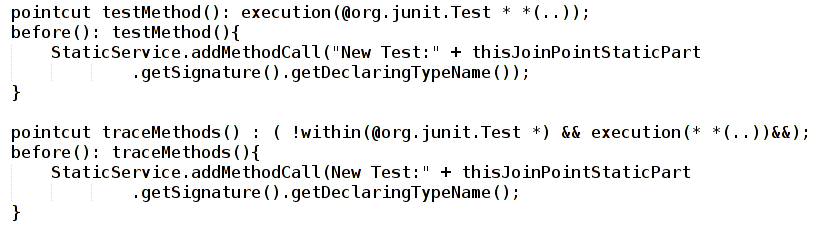
\includegraphics[width = \textwidth]{aspect.png}
\end{center}
\caption{A simplified point cut within AspectJ. The first pointcut is for when a new test is executed and the second when a new method is executed.}
\label{fig:aspectused}
\end{figure}

\section{Framework}
\label{S:framework}

The spectrum of every test has to be compared to that of every other test in order to identify redundant test cases. The metrics identified become computationally heavy with thousands of test cases containing a spectrum consisting of tens of thousands of methods calls. To perform an analysis on that scale would take several days. A pipeline combined with time reduction strategies was determined to be the best solution.

A pipeline approach is shown in Figure \ref{fig:pipeline}. The analysing stages can be set by the user within a properties file, where they can select the spectra type, analysis metric to use and level of redundancy for each. This allows execution of reduction strategies before executing more computationally heavy analysis.

\begin{figure}[h]
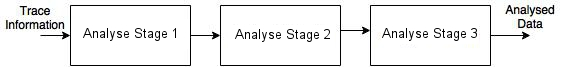
\includegraphics[width=\textwidth]{Pipeline.jpg}
\caption{Trace information goes in at the start of the pipeline. After each stage there will be a reduction of comparisons that the next stage has to complete. The last stages should be the most computationally heavy.}
\label{fig:pipeline}
\end{figure}

There were two approaches that were used to reduce the amount of analysis time. They were - implementing a heuristic and using concurrent execution. 

The heuristic looked at the set spectra of method calls, rather than a list. This meant the number of comparisons decreased. Using a 99 percent similarity for the heuristic on the wyc package of Whiley, this decreased the comparisons that the last had to do from 90,902 to 38.

The following illustrates an example of this.

$K,I,T,C,H,E,N \neq K,I,T,E,N,Z $

In this case, the two test cases would not be redundant due to them having a large difference in method calls.

$K,I,T,C,H,E,N \approx K,I,T,C,H,N$

There is a chance that these two may be redundant so it implies more computational heavy analysis should be done, such as analysing the list spectra or calling context. 

Concurrent execution was implemented by splitting the test cases up into 8 different parts, each part knew the test cases that it had to compare. A new thread was run to execute the comparisons, making the implementation relatively easy. The concurrent execution lead to a decrease in roughly 2 times the time taken to analyse the spectra's but lead to a trade off in an increased memory usage. This meant concurrent execution was only usable for the smaller bench marks.
Another issue was that for each analysis of a benchmark, the tests had to be rerun, this could take several hours. The solution was to save the spectra data to disk. This ensured that a distributed grid system, explored later, can be used to analyse the data.

\section{Benchmarks}
\label{S:bench}
Suitable benchmarks had to be found to test the different metrics on. They were located by looking at popular java framework's, Github repositories and David Pearce's personal projects. The benchmarks had to meet a criteria where they were Java based, had reasonable number of tests (40+) and were open source. Although there were over ten potential benchmarks, the ability to use them depended on their build process. If they used Maven, it was difficult to create a jar that contained the tests and often meant that the amount of effort needed to get a working benchmark was higher than the benefit from it. This eliminated several potential benchmarks and left the Ant and Gradle built projects. In Table \ref{large_test} are the large bench marks used. These involved bench marks that required more than \todo{TODO} number of comparisons. In Table \ref{small_test} are the smaller bench marks used. 

A variety of test types and sizes of the benchmarks were examined. A range of sizes were used in order to fully evaluate the framework. Although the framework and method execution details is more aimed toward larger test suites, it would be expected that they will give the same performance in relation to large test cases with the metrics and spectra's used. A range of test types were also chosen, David J Pearce's projects contain end to end tests which run through a whole module at once, while the others attempt to test units of code at a time. Having a range of test types gives a wider evaluation view and gives insight into potential situations where method details may not be accurate in identifying redundant test cases.

For the larger benchmarks that produced up to 100,000 method calls per test, they required a large amount of memory to store it while the tests were running. Without the use of a database, this limited the number of test cases that could be collected. Whiley and Ant were the benchmarks that did not have all there tests executed.  

\begin{table}[]
\centering
\caption{Large Test Suites}
\label{large_test}
\begin{tabular}{|l|l|l|l|}
\hline
{\bf Benchmark}       &  {\bf Number of Tests} & {\bf Type of tests} & {\bf Authors}   \\ \hline
Whiley - Wyc Valid         &       &    End to End      & David J Pearce          \\ \hline
Spring - Core   &       &    Unit Tests      & Community \\ \hline
Metric-x - Core &       &    Unit Tests      & Community \\ \hline
Jasm              &             &    End to End      & David J Pearce \\ \hline

\end{tabular}
\end{table}

\begin{table}[]
\centering
\caption{Small Test Suites}
\label{small_test}
\begin{tabular}{|l|l|l|l|}
\hline
{\bf Benchmark}   & {\bf Number of Tests} & {\bf Type of tests} & {\bf Authors}  \\ \hline
Ant             &       &    Unit Tests      & Community \\ \hline
Imcache &           &    End to End        & Community \\ \hline
\end{tabular}
\end{table}

